%%%%%%%%%%%%%%%%% 1. lesson
\chapter{Úvodní motivační úlohy ze~spolehlivosti, medicíny, biologie, ekonometrie, experimentální fyziky.}
Ve statistice provádíme experimenty, abychom získali nějaký užitek, případně abychom mohli předvídat budoucí děje. 

\begin{example}[Požár lesa ve~Španělsku]~
	 \begin{enumerate}[a)]
		\item Abychom mohli předvídat budoucí požáry lesa, musíme si nejprve rozmyslet, jestli jsou požáry náhodné, tedy jestli je daná veličina deterministická, nebo stochastická úloha. 
		\item V~tom případě ale potřebujeme model, který by úlohu popisoval. V~rámci toho modelu musíme zkoumat faktory ovlivňující požáry lesa. Těch je však mnoho, a~proto musíme vybrat ty relevantní. 
		\item Dále potom záleží na~struktuře dat. Vezmeme $p$ jako pravděpodobnost, že v~lese vznikne požár. Potom logistický model pro~tuto pravděpodobnost vypadá jako
		$$ p=\frac{\e{\alpha_1 h+\alpha_2t+\alpha_3x}}{1+\e{\alpha_1 h+\alpha_2 t+\alpha_3 x}}, $$
		kde $h$ je vlhost, $t$ teplota a~$x$ stupeň péče o~les.
		\item Snažíme se~nyní odhadnout parametry $\walpha_1,\walpha_2,\walpha_3$. na~základě dostupných dat.
		\item Dále musíme ověřit tento model na~reálné situaci.
	\end{enumerate} 
\end{example}
\begin{example}[Capture-Recapture] V~rybníce je $N$ ryb. Abychom tento počet zjistili, aniž bychom museli vylovit celý rychník, vylovíme pouze $r$ ryb, označíme je a~pustíme zpět do~vody. Dále počkáme, až budou ryby rovnoměrně rozmístěny a~vylovíme $s$ ryb. Z~nich bude $x$ značit počet označených ryb.
	
Rozdělení $x$ je potom $X\sim f_X(x)=\frac{\binom{r}{x}\binom{N-r}{s-x}}{\binom{N}{s}}\sim\mathrm{Hyp}(N,r,s)$. Nyní nám jde o~to odhadnout, jak vypadá $\widehat{N}$ jako odhad počtu ryb v~rybníce. Po~krátké úvaze dospějeme k~tomu, že $\widehat{N}=\frac{rs}{x}$.
\end{example}
\begin{example}[Analýza dat o~přežití]
	Mějme $X\geq0$ jako čas do~poruchy (ale i~něčeho pozitivního). Pokud tento problém řešíme stochasticky, máme rozdělení $X\sim \FF_X,f_X$ a~hledáme $\EE X=\t$, kterou značíme i~jako MTTF (\textit{mean time to failure}). Zavedeme dále \textbf{intenzitu poruch} jako $r_X(x)=\frac{f_X(x)}{1-\FF_X(x)}$. Úkolem je potom nalézt $\widehat{\t}$.
\end{example}
\begin{example}[MEX] Představme si počítačovou síť, kde máme za~úkol kontrolovat switch. Obecně o~jednotlivých uživatelích sítě nevíme nic (nevíme, že zrovna dneska bude někdo stahovat filmy apod.) Označme $X_i \sim \NN$ jako průtok dat od~$i$-tého uživatele. Potom chceme mít pod~kontrolou pravděpodobnost přetečení switche, tedy $\p{\sumin X_i>C_s}<\e{-\gamma}$ (např. $10^{-10}$, což je velice nepravděpodobné). Zabýváme se~tedy jevy, které se~dějí velice zřídka, ale které by mohli mít i~vážný dopad, např. u~povodní. 
\end{example}
\begin{example}[Ekonometrie]
	Víme, že změna mzdy souvisí se~změnou ceny komodity, tedy $\Delta M \stackrel{?}{\leftrightarrow}\Delta C$ (např. $\Delta C=\alpha+\beta(\Delta M)^2+\gamma\ln\Delta M+\epsilon$). Abychom mohli takový vztah odhadnout, potřebujeme data z~minulosti $\big(\Delta M_i,\Delta C_i\big)_{i=1}^n$. Z~toho pak lze odhadnout $\walpha,\wbeta,\wgamma$. Deterministický přístup by byl použít např. lineární regresi. Pokud však bude součástí zadání předpovědět hodnotu v~místě, které nikdy nebylo k~dispozici, nemůžeme si být jisti výsledkem, viz obr.\ref{fig:overfitting}. Cílem je odhadnout $\epsilon$, což můžeme například pomocí CLT jako $\epsilon=\sumin \epsilon_i\sim\AN$.
\end{example}

\begin{figure}[h]
	\centering
	\begin{tikzpicture}[line cap=round,line join=round,>=triangle 45,x=6.0cm,y=6.0cm]
	\clip(-0.26,-0.05) rectangle (1.5,0.68);
	\draw [color=green!45!black](0.75,0.21) node[anchor=north west] {Přeučení};
	\draw [color=red!65!black](0.12,0.45) node[anchor=north west] {Nedostatečné naučení};
	\draw [color=blue!55!black](0.80,0.34) node[anchor=north west] {Skutečná závislost};
	\draw (0,-0.05) -- (0,0.68);
	\draw [domain=-0.26:1.28] plot(\x,{(-0-0*\x)/1});
	\draw[line width=1pt,color=red!65!black] plot[raw gnuplot, id=func0] function{set samples 10000; set xrange [-0.16:1.18]; plot 0.18*x+0.22};
	\draw[line width=1pt,color=blue!55!black] plot[raw gnuplot, id=func1] function{set samples 10000; set xrange [-0.16:1.18]; plot 1.35*x**2-1.06*x+0.31};
	\draw[line width=1pt,color=green!45!black] plot[raw gnuplot, id=func2] function{set samples 10000; set xrange [-0.16:1.18]; plot 1476.55*x**8-5318.13*x**7+7495.45*x**6-5161.41*x**5+1738.28*x**4-227.24*x**3-4.93*x**2+2.01*x+0.25};
	\begin{scriptsize}
	\fill [color=black] (0.7,0.16) circle (3.0pt);
	\fill [color=black] (0.65,0.13) circle (3.0pt);
	\fill [color=black] (-0.09,0.35) circle (3.0pt);
	\fill [color=black] (0.03,0.3) circle (3.0pt);
	\fill [color=black] (0.14,0.26) circle (3.0pt);
	\fill [color=black] (0.2,0.18) circle (3.0pt);
	\fill [color=black] (0.26,0.17) circle (3.0pt);
	\fill [color=black] (0.98,0.62) circle (3.0pt);
	\fill [color=black] (0.93,0.48) circle (3.0pt);
	\fill [color=black] (0.7,0.16) circle (3.0pt);
	\fill [color=black] (0.65,0.13) circle (3.0pt);
	\fill [color=black] (-0.09,0.35) circle (3.0pt);
	\fill [color=black] (0.03,0.3) circle (3.0pt);
	\fill [color=black] (0.14,0.26) circle (3.0pt);
	\fill [color=black] (0.2,0.18) circle (3.0pt);
	\fill [color=black] (0.26,0.17) circle (3.0pt);
	\fill [color=black] (0.98,0.62) circle (3.0pt);
	\fill [color=black] (0.93,0.48) circle (3.0pt);
	\end{scriptsize}
	\end{tikzpicture}
	\caption{Příklad přeučení a~nedostatečného naučení u~kvadratických dat.}
	\label{fig:overfitting}
\end{figure}




$$ \mathcal{F}=\big\{ f(x,\t):\t\in\Theta\subset\R^k \big\} $$
$X_i~iid~f$, kde $f_\textbf{X}=\prod f_{X_i}$. $\widehat{\t}$ na~základě $\textbf{x}$ (rozhodnutí o~$\t$). Znáhodníme parametr $\t$, kde $\t\sim\pi(\t)$.
\begin{theorem}[Bayesova] 
	Mějme $(H_k)_{k=1}^{n,+\infty}$ jako úplný rozklad $\Omega,~A~\in \Aa , ~\PP(A)>0$. Potom $\forall k\in\N$ platí, že 
	\[
	\PP(H_k|A)=\frac{\PP(A|H_k)\PP(H_k)}{\sum\limits_{j=1}^{n,+\infty}\PP(A|H_j)\PP(H_j)}
	\]
	\begin{proof}
		$$\PP(H_k|A)=\frac{\PP(H_k\cap A)}{\PP(A)}=\frac{\PP(A|H_k)\PP(H_k)}{\sum\limits_{j=1}^{n,+\infty}\PP(A|H_j)\PP(H_j)}$$
	\end{proof}
\end{theorem}
\begin{theorem}
	Mějme $X,Y$ jako náhodné veličiny s~$f_{X,Y}$. Pak
	$$ f(y|x)=\frac{f(x|y)g(y)}{\int_{\mathcal{Y}}f(x|y)g(y)dy}. $$
\begin{proof}
$$ f(y|x)=\frac{f_{X,Y}(x,y)}{f(x)}=\frac{f(x|y)g(y)}{\int_{\mathcal{Y}}f(x|y)g(y)dy} $$
\end{proof}

\end{theorem}
%%%%%%%%%%%%%%%%%%%% 2. lesson
\begin{remark}
	Bayesova věta... znáhodnění $\t$. Máme třídu hustot $\mathcal{F}=\big\{f(x,\t):\t\in\Theta\subset\R^k\big\},~\t\sim\pi(\t)$. Dále $X\sim f(x|\t)\Rightarrow \X=(X_1,...,X_n)~iid~f_\X(\textbf{x}|\t)$.
	
	Z toho vyplývá, že $\phi(\textbf{x},\t)=f(\textbf{x}|\t)\pi(\t)$, $m(\textbf{x})=\int\phi(\textbf{x},\t)\d \t=\int f(\textbf{x}|\t)\pi(\t)\d\t$ jako marginální rozdělení $\X$. 
	$$ \pi(\t|\textbf{x})\stackrel{B}{=}\frac{\phi(\textbf{x},\t)}{m(\textbf{x})}=\frac{f(\textbf{x}|\t)\pi(\t)}{\int_\Theta f(\textbf{x}|\t)..........} $$
	\begin{itemize}
	\item 	$\pi(\t)$ nazýváme \textit{apriorní hustota}
	\item   $\pi(\t|\textbf{x})$ nazýváme \textit{aposteriorní hustota}
	\item znáhodnění $\theta$ je tedy způsob, jak sumarizovat dosažitelnou informaci o $\theta$
	\end{itemize}

\begin{center}
    
    \begin{tikzpicture}
    \node[inner sep=0pt] (pic) at (0,0)
    {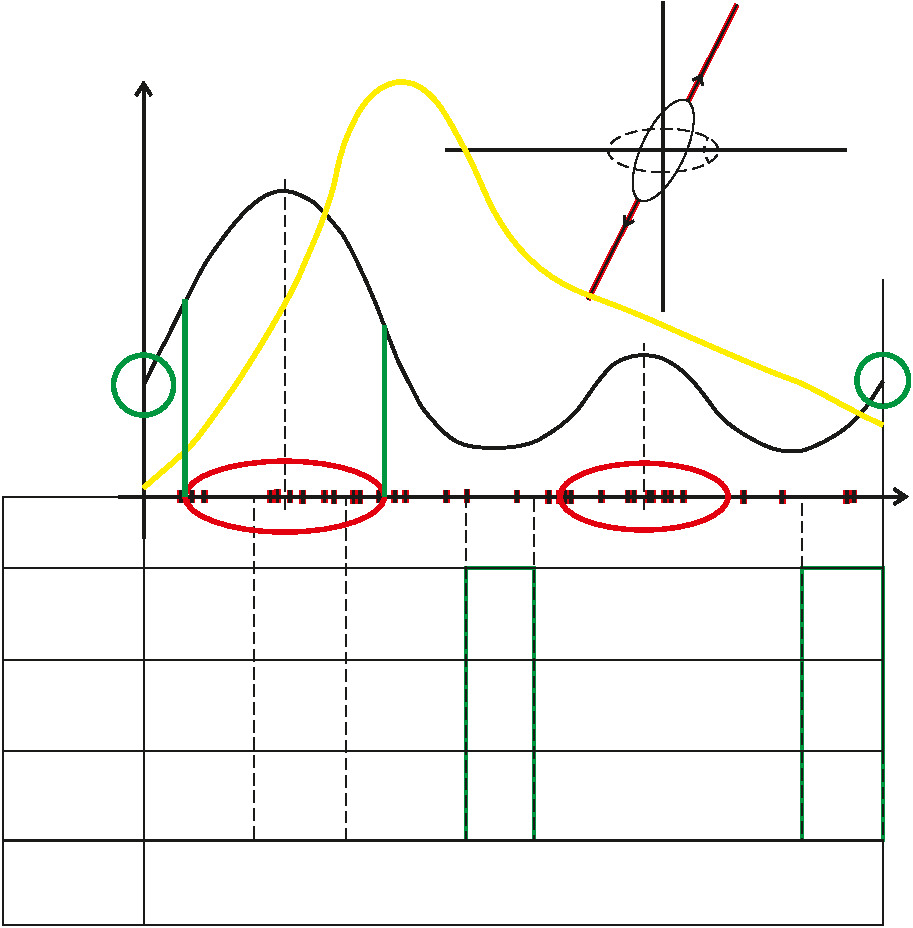
\includegraphics[width=10cm]{pictures/picture_1_3.pdf}};
    \draw [color=red](-3.5,-1.3) node[anchor=north west] {Dodelat popisky? Budeme chtít i tento příklad?};
    \end{tikzpicture}
\end{center}
	
\end{remark}


$\pi(\t)$ lze určit na základě:\begin{enumerate}[a)]
	\item objektivní informace, tj. znalost z~předchozích úloh (z minulosti),
	\item subjektivní informace (znalost experta, naše znalost, ...),
	\item kombinace a) a~b) ($C=\alpha_1\pi_1(\t)+\alpha_2\pi_2(\t)$), případně více a) nebo více b)
	\item neurčitost (neznalost)
\end{enumerate}

-------------PIC03----------------

\begin{remark}
	Tímto způsobem by se~dalo pojmout i~strojové učení. To bere nějaká trénovací a~testovací data, kde na~trénovacích datech dochází k~učení modelu a~na~testovacích datech (která nebyla použita při~trénování) pak vyhodnocuje, jak moc daný model funguje.
\end{remark}
Takto víceméně funguje rozhodování, která děláme. 
$$ \pi(\t)\stackrel{\text{data}}{\longrightarrow}\pi_n(\t|\textbf{x})\to \widehat{\t}_B=\EE{\pi(\t|\textbf{x})}$$
Chtěli bychom, aby byl náš odhad $\widehat{\t}_B\big( \pi_s(\t|\textbf{x}) \big)$ s~rostoucím $n\to+\infty$ stále méně ovlivněn $\pi(\t)$.
\begin{remark}
Při určení odhadu parametru $ \theta $ nemusí být vždy nejvhodnější volbou $ \theta_{\text{MLE}} = \text{argmax}[\pi(\t|\textbf{x})]$. Můžou nastat případy, kdy je střední hodnota aposteriorní hustoty pravděpodobnosti $ \pi $ vhodnější.
\begin{center}
    
    \begin{tikzpicture}
    \node[inner sep=0pt] (pic) at (0,0)
    {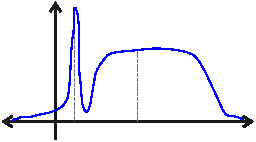
\includegraphics[width=10cm]{pictures/picture_2_1.pdf}};
    \draw [color=black](-2.5,-2) node[anchor=north west] {$ \widehat{\t}_{\text{MLE}} $};
    \draw [color=black](0.2,-2) node[anchor=north west] {$ \widehat{\t}_{\text{B}} $};
    \draw [color=blue](2.8,1.2) node[anchor=north west] {$ \pi(\t|\textbf{x}) $};
    \end{tikzpicture}
\end{center}
\end{remark}


\begin{example} --zde by to chtělo asi lepší popis--
	Představme si, že máme biliárový stůl a dva hráče, kteří mezi sebou hrají. První hráč dostane kouli na pozici (1) s pravděpodobností $p$, která leží mezi 0 a 1. Druhý hráč chce poté odhadnout místo, kde se koule prvního hráče nachází, čili chce dostat odhad $\widehat{p}=?$ na základě $n$ šťouchů, o kterých víme, že se buďto dotkly koule, či nikoliv. 
	
	statistika: máme $n$ šťouchů s~rovnoměrným rozdělením. Označme $X$ jako počet neťuků. $X(\omega)=\textbf{x}$, což jsou data, která máme k~dispozici a~ptáme se~na~odhad $\widehat{p}=?$.
	
	\begin{figure}[h]
	\centering  
    \begin{tikzpicture}
    \node[inner sep=0pt] (pic) at (0,0)
    {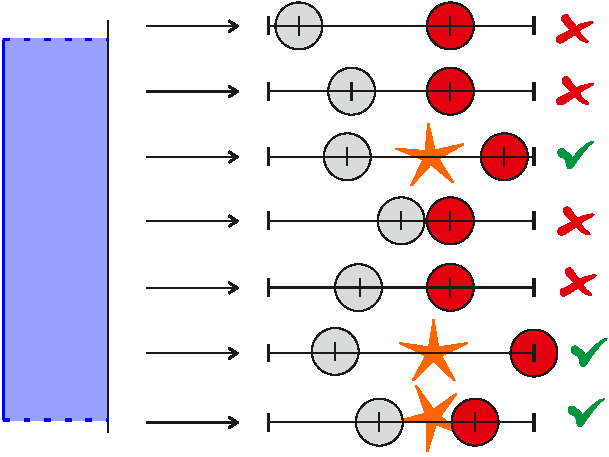
\includegraphics[width=8cm]{pictures/picture_2_2.pdf}};
    \draw [color=blue](-4.0,0.4) node[anchor=north west] {$ \text{U}(0,1) $};
    \draw [color=black](-0.75,3.5) node[anchor=north west] {$ 0 $};
    \draw [color=black](2.65,3.5) node[anchor=north west] {$ 1 $};
    \draw [color=black](1.6,3.5) node[anchor=north west] {$ p $};
    \draw [color=black](4.6,0.4) node[anchor=north west] {$ \text{Bi}(n,p) $};
    \draw [color=black](-1.9,3.2) node[anchor=north west] {$ \text{X}_{1} $};
    \draw [color=black](-1.9,2.35) node[anchor=north west] {$ \text{X}_{2} $};
    \draw [color=black](-1.9,1.5) node[anchor=north west] {$ \text{X}_{3} $};
    \draw [color=black](-1.9,0.65) node[anchor=north west] {$ \text{X}_{4} $};
    \draw [color=black](-1.9,-1.9) node[anchor=north west] {$ \text{X}_{n} $};
    \end{tikzpicture}
	\caption{Kulečníkový stůl.}
\end{figure}
	
	\begin{enumerate}[a)]
		\item Předpokládejme, že 1. hráč je uniformní. Potom $p\sim\pi(p)=1$ na~$(0,1)$ (podle principu neurčitosti). Potom
		$$ X\sim\Bi(n,p)=f(x|p).$$
		Dále pak 
		$$ \pi(\t|x)=\frac{f\cdot\pi}{\int_0^1 f\pi\d p}=\frac{\binom{n}{x}p^x(1-p)^{n-x}\cdot 1}{\int_0^1 \binom{n}{x}p^x(1-p^{n-x}\cdot1 \d p)}=\mathrm{Beta}(x+1,n-x+1).$$
		Z toho vyplývá, že
		$$ \widehat{\t}_B=\widehat{p}_B=\EE{p|x}=\int...=\frac{x+1}{n+2}.$$
		Potom se~můžeme ptát, jaké je $p$, pokud známe $\textbf{x}$. Klasický odhad by byl ve~tvaru $\widehat{p}_{\mathrm{ML}}=\frac{x}{n}$.
		\item $\pi(\t)=\pi(p)=\mathrm{Beta}(\alpha,\beta)$ Z~toho pak 
		\[
		\begin{split}
		\pi(p|x)&=\frac{f\cdot\pi}{\underbrace{\int f\pi}_c}=\frac{1}{c}\binom{n}{x}p^x(1-p)^n\cdot \frac{1}{B(...)}p^{\alpha-1}(1-p)^{\beta-1}=\frac{1}{c'}p^{x+\alpha-1}(1-p)^{n-x+\beta-1}=\\&=\mathrm{Beta}(x+\alpha,n-x+\beta).
		\end{split}
		\] 
		Dále
		$$ \widehat{p}_B=\EE{\mathrm{Beta}(x+\alpha,n-x+\beta)}=\frac{x+\alpha}{n+\alpha+\beta}\doteq\frac{x}{n} = \widehat{p}_{ML} ~~~\text{pro velká \textit{n}, tedy i velká \textit{x}}$$
	\end{enumerate}
\end{example}

\begin{center}
    
    \begin{tikzpicture}
    \node[inner sep=0pt] (pic) at (0,0)
    {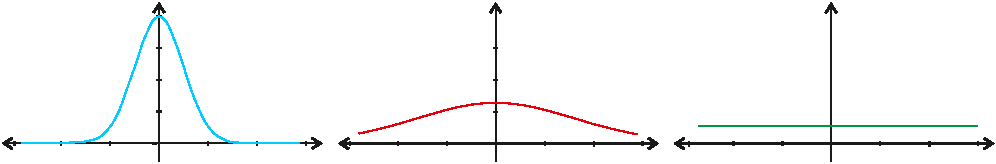
\includegraphics[width=10cm]{pictures/picture_2_4.pdf}};
    \draw [color=black](0,-4.7) node[anchor=north west] {$ c $};
    \draw [color=black](0,-1.6) node[anchor=north west] {$ \mu_{0} $};
    \draw [color=black](0,2.7) node[anchor=north west] {$ \mu_{0} $};
    \draw [color=black](3,4) node[anchor=north west] {$ \sigma^{2} = 1 $};
    \draw [color=black](3,0) node[anchor=north west] {$ \sigma^{2} = 10 $};
    \draw [color=black](3,-4) node[anchor=north west] {$ \sigma^{2} \rightarrow \infty $};
    \end{tikzpicture}
\end{center}

$\pi(\t)=c\neq0$ konstantní, takže $\pi(\t)$ můžeme volit tak, aby $\int_\Theta\pi(\t)=+\infty$.
\begin{define}[Nevlastní hustota (apriorní)] Definujeme apriorní nevlastní hustotu jako hustotu $\pi(\theta)$ takovou, že $$ \int\limits_{\Phi}{\pi(\theta)} = +\infty,$$  avšak 
	$$\pi(\t|x)=\frac{f\cdot \pi}{\int f\pi\d\t}$$ je stále regulární hustotou. Nevlastní hustota $\pi(\theta)$ tedy stále nese apriorní informaci o $\theta$.
\end{define}
\begin{example}\begin{enumerate}[a)]
		\item 
	Mějme $X\sim f(x|\mu)=\NN(\mu,1)$, kde $\mu\in\R$. Dále nechť $\pi(\mu)=c\neq0$. Potom$$ \pi(\mu|x)=\frac{f\cdot \pi}{\int_{-\infty}^{+\infty}\frac{1}{\sqrt{2\pi}}\e{-\frac{1}{2}(x-\mu)^2}c\d\mu}=\frac{\e{-\frac{1}{2}(\mu-x)^2}}{\sqrt{2\pi}}\sim\NN(x,1).$$
	Dále pak 
	$$\widehat{\mu}_B=\EE{\NN(x,1)}=x=\widehat{\mu}_{\mathrm{ML}}.$$
	\item Nechť $f=\NN(0,1)$ a~$\pi(\mu)=\NN(0,10)$.
	
	------------------PIC07---------------
	
	Pojďme nyní udělat apriorní odhad $\mu$, tedy $\widehat{\mu}_{\mathrm{apr.}}=\EE{\NN(0,10)}=0$. $X=x...f_X$. Dále
	$$ \pi(\mu|x)=\frac{1}{c}f\cdot\pi=\frac{1}{c}\e{-\frac{1}{2}(x-\mu)^2}\e{-\frac{1}{20}(\mu-o)^2}=\frac{1}{c}\e{-\frac{11}{20}(\mu-\frac{10}{11}x)^2}$$ s~rozdělením $\NN\left(\frac{10}{11}x,\frac{10}{11}\right)$.
	Pro odhad $\mu$ pak platí, že
	$$\widehat{\mu}_B=\EE{\pi(\mu|x)}=\int\frac{1}{c}\e{-\frac{11}{20}(\mu-\frac{10}{11}x)^2}\d\mu=\frac{10}{11}x.$$ 
	
	HPD (High Posterior Density) region
	
	------------------PIC08-------(i s~tou rovnicí, tu bych dal do obrázku)--------
	
	Zkoumáme tedy hypotézu $\hypothesis{\t\in\Theta_0}{\t\notin\Theta_0}$. Máme k~dispozici $\X$ a k ní příslušnou statistiku $T(\X)$, kde $T(\X)\sim\FF_T$. Testujeme tedy na základě kritické oblasti $W_\alpha=\big\{ |T(\X)|<K_\alpha \big\}$. Toto byl přístup doposud. Nyní nám ale Bayesova věta říká, že pokud je $\t$ znáhodněný parametr, tak potom můžeme přímo vyjádřit pravděpodobnost (ať už apriorní, či aposteriorní), že platí $H_0$, a to následovně
	$$\PP(H_0) = \PP(\theta \in \Theta_0),$$
	jelikož na parametr $\theta$ nahlížíme jako na náhodnou veličinu. Pravděpodobnost $\PP(\theta \in \Theta_0)$ lze, jak již bylo zmíněno, počítat vzhledem k apriornímu i aposteriornímu rozdělení $\theta$.
	\end{enumerate}
\end{example}
